\section{Example: Mergesort}
\label{sec:mergesort}

We now consider another example of fine-grained concurrency, and build a
circuit to sort a stream of integers, based on the Mergesort algorithm.  The
circuit inputs a steam of |Int|s (with the end of stream signalled by the
channel closing), and then outputs a sorted version of that stream (and closes
the channel to indicate the end of the stream).  The circuit is not the most
practical way to sort numbers, but it illustrates various ideas.

More precisely, we will write a  definition with the following signature
%
\begin{scala}
  def mergesort(in: ??[Int], out: !![Int]): ThreadGroup = ...
\end{scala}
%
The function will produce a |ThreadGroup| that, when run, performs the
sorting.  The Mergesort algorithm is recursive, so the |mergesort| function
will also be recursive.

Suppose the input stream is empty.  Then |mergesort| should just close its
output channel to signal an empty output stream.  Similarly, if the input
stream contains a single value~|x1|, then |mergesort| should output~|x1| and
then close its output channel.  This can be achieved using the following
outline:
%
\begin{mysamepage}
\begin{scala}
  def mergesort(in: ??[Int], out: !![Int]): ThreadGroup = thread("mergesort"){
    var x1 = -1; var x2 = -1
    attempt{ 
      x1 = in?()
      attempt{
        x2 = in?()
        ...   // Sort stream starting with £x1£ and £x2£.
      }{ out!x1; out.endOfStream() } // Received only £x1£.
    }{ out.endOfStream() } // Received empty stream.
  }
\end{scala}
\end{mysamepage}
%
The command |attempt{p}{q}| acts like~|p|, but if that throws a |Stopped|
exception, it executes~|q|.  Thus if the initial attempt to input |x1| on |in|
fails, the function signals |endOfStream| on |out|; and if the attempt to
input~|x2| on~|in| fails, the function outputs~|x1| and then signals
|endOfStream| on |out|.

We now consider the case where the input stream contains at least two values,
starting with~|x1| and~|x2|.  We create two recursive |mergesort|
threads that will each sort about half of the inputs.  In addition, a
controller thread ties things together.  The controller:
%
\begin{itemize}
\item Passes the first two values, |x1| and |x2|, to the two recursive
  |mergesort|s;

\item Continues  to input on |in|, passing values alternately to the  recursive
  |mergesort|s;

\item When |in| is closed, closes the channels to the recursive |mergesort|s
  to signal the end of their input streams;

\item Receives the outputs from the recursive |mergesorts|, and merges them
  together on |out|.
\end{itemize}
%
The following diagram illustrates how the controller communicates with the
recursive |mergesort| processes.
%
\begin{center}
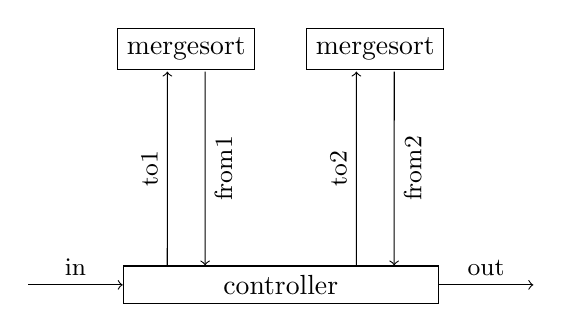
\begin{tikzpicture}[xscale = 1.2]
\draw (0,0) node[draw, minimum width=40mm] (controller) {\scalashape controller};
\draw[->] (controller.west) ++ (-1,0) -- 
   node[above]{\scalashape\small in} (controller.west);
\draw[<-] (controller.east)++(1,0)  -- 
   node[above]{\scalashape\small out} (controller.east);
%
\draw (controller) ++ (-1,3) node[draw] (rec1) {\scalashape mergesort};
\draw (rec1.south)++(-0.20,0.1) node (rec1In) {};
\draw[->] (controller.north) ++ (-1.201,0.0) -- 
  node[above,sloped] {\scalashape\small to1} (rec1In);
% Note: the 0.001 difference between x-coords is to get the label on the right
% side.
\draw (rec1.south)++(0.2,0.1) node (rec1Out) {};
\draw[<-] (controller.north) ++ (-0.801,0) -- 
  node[below,sloped] {\scalashape\small from1} (rec1Out);
%
\draw (controller) ++ (1,3) node[draw] (rec2) {\scalashape mergesort};
\draw (rec2.south)++(-0.2,0.1) node (rec2In) {};
\draw[->] (controller.north) ++ (0.8,0.0) -- 
  node[above,sloped] {\scalashape\small to2} (rec2In);
\draw (rec2.south)++(0.2,0.1) node (rec2Out) {};
\draw[<-] (controller.north) ++ (1.2,0) -- 
  node[below,sloped] {\scalashape\small from2} (rec2Out);
\end{tikzpicture}
\end{center}

%%%%%

The code in Figure~\ref{fig:mergesort} implements this strategy.  
%% (We describe
%% below the |merge| function that merges the streams from the recursive
%% threads.) 
Thus, when the input stream contains at least two elements, the
|mergesort| function runs the parallel composition of the controller and the
results of two recursive calls to |mergesort|.

\begin{figure}
\begin{scala}
  /** Merge sorted streams received on £in1£ and £in2£ into a single sorted
    * stream on £out£. */
  private def merge(in1: ??[Int], in2: ??[Int], out: !![Int]) = {
    var x1 = in1?(); var x2 = in2?(); var closed1 = false; var closed2 = false
    while(!closed1 && !closed2){
      if(x1 <= x2){ out!x1; attempt{ x1 = in1?() }{ closed1 = true } }
      else{ out!x2; attempt{ x2 = in2?() }{ closed2 = true } }
    }
    if(closed2){ out!x1; repeat{ out!(in1?()) } }
    else{ assert(closed1); out!x2; repeat{ out!(in2?()) } }
    out.endOfStream()
  }

  def mergesort(in: ??[Int], out: !![Int]): ThreadGroup = thread("mergesort"){
    var x1 = -1; var x2 = -1
    attempt{ 
      x1 = in?()
      attempt{
        x2 = in?()
        val to1, to2, from1, from2 = new UnboundedBuffChan[Int]
        def controller = thread("controller"){
          to1!x1; to2!x2
          repeat{ to1!(in?()); to2!(in?()) }
          to1.endOfStream(); to2.endOfStream()
          merge(from1, from2, out)
        } // End of £controller£.
        // Put the system together and run it.
        run( controller || mergesort(to1, from1) || mergesort(to2, from2) )
      }{ out!x1; out.endOfStream() } // Received only £x1£.
    }{ out.endOfStream() } // Received empty stream.
  }
\end{scala}
\caption{The concurrent Mergesort program.}
\label{fig:mergesort}
\end{figure}

The first part of the definition of the controller is straightforward.  The
|merge| function repeatedly holds two values that it received from the two
recursive |mergesort|s; it outputs the smaller, and inputs again from the
relevant recursive |mergesort|.  However, the definition is made harder by the
fact that when one of its input streams is closed, it will still be holding a
value it received on the other input stream: it needs to output that value,
and also deal with any remaining values in the non-closed stream.  The code
does this by maintaining two boolean variables.  The variable |closed1| is
true if |in1| has been detected as closed; otherwise |x1| holds the last value
read from |in1|, which has not yet been output.  A similar property holds for
|closed2|, |x2|, and~|in2|.

\begin{instruction}
Make sure you understand the code in Figure~\ref{fig:mergesort}.
\end{instruction}

%%%%%  

We now consider testing.  Testing is an important part of programming.  But
testing is particularly important for concurrent programs, because they tend
to be somewhat harder than sequential ones.

A fairly general strategy for testing a concurrent program is to generate some
random data, run the concurrent program on it, run a corresponding sequential
program on it, and check that the two give the same answer.  This can be
repeated many times.  Of course, this assumes that we have a correct
sequential program for the same problem, but that's normally not too
difficult.  In fact, this strategy is also useful for testing sequential
programs, where we have a simple implementation that we are sure is correct,
but we want to test a more sophisticated implementation against it.

\begin{figure}
\begin{scala}
  import scala.util.Random
  val MaxSize = 100; val Max = 100
  def doTest = {
    val size = Random.nextInt(MaxSize)
    val xs = Array.fill(size)(Random.nextInt(Max)); val ys = new Array[Int](size)
    val in, out = new SyncChan[Int]
    def sender = thread("sender"){ for(x <- xs) in!x; in.endOfStream() }
    def receiver = thread("receiver"){ 
      var i = 0; repeat{ ys(i) = out?(); i += 1 } 
    }
    run(sender || mergesort(in, out) || receiver)
    assert(xs.sorted.sameElements(ys),
      "Inputs: "+xs.mkString(", ")+"\nExpected: "+xs.sorted.mkString(", ")+
      "\nReceived: "+ys.mkString(", "))
  }

  def main(args: Array[String]) = {
    for(i <- 0 until 1000){ doTest; if(i%10 == 0) print(".") }
    println()
  }
\end{scala}
\caption{Testing code for the {\scalashape mergesort} function.}
\label{fig:mergesort-test}
\end{figure}

The code in Figure~\ref{fig:mergesort-test} implements this idea.  The
|doTest| function performs a single test.  If uses an array |xs| of
size~|size|, where |size| is picked randomly in the range\footnote{We use the
  notation $\interval{a}{b}$ to represent the numbers in the half-open
  interval from $a$ up to but not including~$b$.}
$\interval{0}{\sm{MaxSize}}$; each element of |xs| is picked randomly in the
range $\interval{0}{\sm{Max}}$.  The |sender| thread sends the elements
of~|xs| to the |qSort| network on the |in| channel, then signals the end of
the stream.  The |receiver| thread receives the outputs from |qSort|, and
stores them in~|ys|.  The final assertion tests whether a sorted version of
|xs| (produced using the |sorted| function from the Scala |Array| class)
contains the same elements as the outputs; if this doesn't hold, it prints
information about the inputs and outputs, to help with debugging.

The |main| function  runs |doTest| many times.
%% %
%% \begin{scala}
%%   for(i <- 0 until 1000){ doTest; if(i%10 == 0) print(".") }
%% \end{scala}
%
It also intermittently prints a dot on the screen; this means that if the
system deadlocks for some reason, we will spot that it has got stuck!

There are several exercises at the end of this chapter that involve building
sorting circuits.  They can be tested in the same way.
%
\begin{instruction}
Study the details of the testing program.
\end{instruction}

%%%%%%%%%%%%%%%%%%%%%%%%%%%%%%%%%%%%%%%%%%%%%%%%%%%%%%%%%%%%

\section{Reasoning About the Order of Actions}

We will sometimes want to reason about the order in which particular
actions---such as memory reads and writes, and sends and receives of
messages---occur.

Consider a particular execution of a program.  We will write $a \prec a'$, to
mean that $a$ necessarily happens before~$a'$.  For example, $a$ and~$a'$
might be events performed by the same thread in that order; or they might,
respectively, be a send and receive on a buffered channel.

We will write $a \preceq a'$ to mean that $a$ happens before, or
simultaneously with, $a'$.  
%
We write $\equiv$ for the equivalence relation induced by~$\prec$:
\[\mstyle
a \equiv a' \iff a \preceq a' \land a' \preceq a.
\]
This means that $a$ and~$a'$ happen at the same time.  For example, they might
actually be the same action.  However, we also treat a send and receive on a
\emph{synchronous} channel as happening at the same time.

For example, consider the following program.
\begin{scala}
  val c = new OnePlaceBuffChan[Unit]
  run(thread{ print("Hello "); c!() } || thread{ c?(); println("world") })
\end{scala}
%
The type |Unit| contains a single value, called the unit value, denoted~|()|.
Thus communications on~|c| do not pass any data, but just send a signal.
%
We can reason about the above program using happens-before notation.  We
represent actions of the program by the corresponding program syntax.  Then in
every execution:
\[
\begin{array}{cl@{\qquad}l}
& \sm{print("Hello ")} \\
\prec & \sm{c!()} & \mbox{(program order for the first thread)} \\
\prec & \sm{c?()} & \mbox{(ordering for a buffered channel)} \\
\prec & \sm{println("world")} & \mbox{(program order for the second thread).}
\end{array}
\]
The order of printing is as we would like. 

If we use a synchronous channel, we can reverse the send and receive:
%
\begin{scala}
  val c = new SyncChan[Unit]
  run(thread{ print("Hello "); c?() } || thread{ c!(); println("world") })
\end{scala}
%
Reasoning as before:
\[
\begin{array}{cl@{\qquad}l}
& \sm{print("Hello ")} \\
\prec & \sm{c?()} & \mbox{(program order for the first thread)} \\
\equiv & \sm{c!()} & \mbox{(ordering for a synchronous channel)} \\
\prec & \sm{println("world")} & \mbox{(program order for the second thread).}
\end{array}
\]
In this case, the communication on~|c| acts as a synchronisation between the
two threads, without passing any data.
  
Formally, $\preceq$ is a preorder (i.e.,~a transitive, reflexive order) such
that:
%
\begin{itemize}
\item
If $a$ and $a'$ are actions of a single thread, and $a$ precedes $a'$ in
program order, then $a \prec a'$;

\item
If $a$ is a send and $a'$ is the corresponding receive on a buffered channel,
then $a \prec a'$;

\item
If $a$ is a send and $a'$ is the corresponding receive on a synchronous
channel, then $a \equiv a'$.
\end{itemize}

Note that some pairs of actions may be unrelated by~$\preceq$.  For example,
consider two actions in different threads, with no intervening channel
communication.  In such cases, the actions can happen concurrently in either
order, so, we need to be sure that either order is acceptable---i.e.~there is
no race condition.

Using this style of reasoning can also be useful for reasoning about the
efficiency of a concurrent program.  Suppose we can find a chain of $n$
ordered actions:
\[
\mstyle
a_1 \prec a_2 \prec \ldots \prec a_n. 
\]
Then we can be sure that the time taken for the program to complete is at
least the time to perform those $n$ actions.  Conversely, suppose we can be
sure that there is no such chain of length longer than~$n$, and suppose we run
the program on hardware such that every thread can run on its own processor,
without being descheduled; then the program will run in time $O(n)$.  Thus
finding the length of the longest such chain can give us an idea of the
running time of the program (modulo the assumption about hardware).

For example, consider the Mergesort program from the previous section.  It is
enough to consider just the actions of sending and receiving messages: between
any consecutive pair of such actions, a thread does $O(1)$ amount of work.
Let's write $A(l)$ for the number of such actions performed on an input stream
of length~$l$.  For simplicity, let's restrict to  cases where $l$ is a
power of~2.  Then we have the following equations:
%
\begin{eqnarray*}
A(1) & = & 2, \\
A(l) & \le & 4l+A(l/2).
\end{eqnarray*}
%
The first equation is straightforward: the one data value is inputted and
outputted.  For the second clause, note that a maximal chain is comprised of:
the controller inputting $l$ values interleaved with $l$ sends of those values
to the recursive threads; $A(l/2)$ actions by a recursive thread; then the
controller receiving $l$ values from the recursive threads interleaved with
$l$ outputs of those values.  In particular, the actions of the two recursive
threads can occur concurrently (we used buffered channels to ensure neither
recursive thread could be held up by the controller not being ready to accept
its outputs).  In fact, the equation gives an upper bound on $A(l)$, as it
doesn't take account of the fact that some actions of the recursive threads
can be concurrent with actions of the controller. 

It is then straightforward to show that $A(l) \le 8l$ (e.g.~via a proof by
induction).  Thus we can potentially sort $l$ inputs in time $O(l)$---unlike
the $O(l \log l)$ time for a sequential program!  This result needs to be
treated with a pinch of salt: the program uses nearly~$2l$ threads, and for
even moderate values for~$l$, we're unlikely to have enough processors for
every thread to run without being descheduled.
